%Version en ligne
\documentclass[12pt,a4paper]{report}
%Version imprimable
%\documentclass[12pt,a4paper,twoside,openright]{report}

% ************************
% * fichier de préambule *
% ************************

% ***** extensions *****
\usepackage[T1]{fontenc}	% Caractères accentués et césure
\usepackage[utf8x]{inputenc}	% Choix de l'encodage
\usepackage{graphicx}		% Paquage pour l'insertion d'images
\usepackage{wrapfig}		% Figures flottantes
\usepackage[french]{babel}	% Support Français
\usepackage{eurosym}		% Signe € qui s'adapte en fonction de la police
\usepackage{fancyhdr}		% En-tête de pages personalisés
\usepackage{color}		% Un peu de couleurs
\usepackage{array}		% Faire des beaux tableaux
% Liens cliquables dans le document
\usepackage[colorlinks=true,linkcolor=black,urlcolor=blue,%
pdftitle={Workshop Space Invaders},pdfauthor={Némunaire}]{hyperref}
\usepackage{amsmath}		% Formules matématiques
\usepackage{listings}           % Mise en forme de code source

% Changement des polices du document
\usepackage{palatino}
\usepackage[sc]{mathpazo}
\linespread{1.05}


% ***** césures particulières *****

\hyphenation{}

% ***** filigrane *****
%\usepackage{eso-pic,rotating}
%\AddToShipoutPicture{%
%\unitlength 1cm
%\put(11,15){%
%\begin{rotate}{45}
%\makebox(0,0){\color{lightgray}\scalebox{3.5}{\Huge BROUILLON}}
%\end{rotate}}
%}

% ***** couleurs perso *****

\definecolor{lightgray}{RGB}{240,240,240}

\definecolor{vert}{RGB}{0,176,80}
\definecolor{verta}{RGB}{79,97,40}
\definecolor{vertb}{RGB}{195,214,155}
\definecolor{vertc}{RGB}{235,241,221}
\definecolor{bleua}{RGB}{31,73,125}
\definecolor{bleub}{RGB}{219,229,241}
\definecolor{rougea}{RGB}{192,80,77}
\definecolor{rougeb}{RGB}{242,220,219}

\definecolor{brown}{RGB}{128,0,0}
\definecolor{blue}{RGB}{0,0,255}
\definecolor{green}{RGB}{0,128,0}
\definecolor{seagreen}{RGB}{69,158,181}


% ***** paramètre de la coloration syntaxique *****
\lstset{language=C++,basicstyle=\ttfamily\footnotesize,%
stringstyle=\ttfamily\color{brown},commentstyle=\color{green},%
%numberstyle=\footnotesize,stepnumber=1,numbersep=7pt,%
backgroundcolor=\color{vertc},frame=single,tabsize=2,breaklines=true,%
breakatwhitespace=false,%
classoffset=0,% Mots clés non reconnus
morekeywords={implicit,override,string,abstract},keywordstyle=\color{blue},%
classoffset=1,% Noms de classes
morekeywords={Value,Convert,Exp,Cst},keywordstyle=\color{seagreen},%
classoffset=0
}

% ***** commandes personnelles *****

\newcommand{\helpbox}[3][bleu]{\vspace{1em}\fcolorbox{#1a}{#1b}{\parbox{.92%
\linewidth}{\hspace{5pt}\textbf{#2~:} #3}}\vspace{0.75em}}
\newcommand{\tp}{workshop}
\newcommand{\Tp}{Workshop}
\newcommand{\svn}{\textsc{svn}}
\makeatletter
\renewcommand{\chapter}{\clearpage%
     \@startsection{chapter}{1}{-0.75em}{\baselineskip}%
     {0.5\baselineskip}{\LARGE\textbf}}
\makeatother
\renewcommand{\thechapter}{\Roman{chapter}}
\renewcommand{\thesection}{\arabic{section}}

% ***** en-têtes et pieds de pages *****
\pagestyle{fancyplain}
	\lhead[\emph{\nouppercase{\leftmark}}]{\emph{\textit{\Tp{} Subversion}}}
	\chead{} 
	\rhead[\emph{\textit{\Tp{} Subversion}}]{\emph{\nouppercase{\leftmark}}}
	\lfoot[]{\small{\textit{GConfs 2010}}}
	\rfoot[\small{\textit{GConfs 2010}}]{}


\begin{document}

\title{
  \vspace{1cm}
  \textbf{\Huge{\Tp{} projet de jeu vidéo \no 1}}\\
  \vspace{1cm}
  
\includegraphics[scale=0.75]{images/logo.png}
}
\author{
  \Large{Pierre-Olivier \textit{Némunaire} \textsc{Mercier} ({\ttfamily mercie\_d})}\\\\
  Avec l'aimable contribution de~:\\
  Ivan \textit{Colona} \textsc{Delalande} ({\ttfamily delala\_i}) pour l'histoire et les règles\\
  Sébastien \textsc{Crozet} ({\ttfamily crozet\_s}) pour l'organisation d'un jeu
}
\date{
  
\includegraphics[scale=0.5]{images/gconfs.png}\\
  \vspace{0.5cm}
  Vendredi 03 décembre 2010
}

% ************************
% *     introduction     *
% ************************
\maketitle

\tableofcontents

% ************************
% *    contenu du doc    *
% ************************

\chapter{Introduction}

\section{Présentation du \tp}

Ce premier \tp{} a pour but principal de vous familiariser avec un logiciel de versionnement. Pour votre premier contact avec ce genre de logiciel, nous avons choisi de vous décrire l'utilisation de \href{http://subversion.tigris.org/}{Subversion} (plus couramment abbrégé par \textsc{svn}) avec le logiciel \href{http://tortoisesvn.tigris.org/}{TortoiseSVN}.

Il existe bien entendu d'autres méthodes pour gérer les versions de votre code, parfois plus complètes, mais très souvent plus complexes à utiliser.\\

La conférence à laquelle vous venez d'assister vous a présenté toutes les informations à connaître pour pouvoir utiliser un gestionnaire de versionnement~; la partie suivante n'est qu'une transcription de ce qui a été dit durant la conférence, si vous avez compris le principe de ce genre de programme, passez directement au chapitre suivant.


\section{Les gestionnaires de versions}

Les logiciels de versionnement ont pour but de garder une trace de chaque modification que vous avez pu effectuer dans une arborescence de fichiers. Lorsque l'on travaille en équipe, chaque utilisateur possède sur son (ou ses !) ordinateur une copie locale du projet sur lequel il pourra effectuer les modifications qu'il voudra. À intervalle régulier, chacun ira récupérer les modifications effectuées par les autres et enverra également les siennes sur un serveur central (appelé \emph{dépôt} ou \emph{repository} en anglais) dans le cas de \svn.

Comme chaque utilisateur envoie ses modifications sur le serveur régulièrement, chacun a dans son répertoire de travail, toujours une version à jour du projet.\\

Mieux encore~: lorsque deux utilisateurs modifient un même fichier, Subversion est capable de fusionner les modifications. Faire ça à l'aide de l'explorateur Windows de façcon régulière à coup de copie et de fusion grossière demande beaucoup plus d'attention, et cela se termine bien souvent par un fichier malencontresement écrasé, source de bug de dernière minute.

\chapter{Histoire et règles}

Pour essayer de reproduire un jeu, il est important de comprendre quelles sont
ses règles et dans quel contexte il est sorti. Cependant, si cette partie vous
ennuie, que vous connaissez déjà tout ou que vous vous en foutez, rien ne vous
empêche de la passer.

\section{Histoire}

\subsection{Version courte}

Taito sort \emph{Space Invaders} en juillet 1978 au Japon sous forme d’une borne
d’arcade et fait un véritable carton.

\subsection{Version romanesque}

Durant la première moitié des années 70, le (petit) monde du jeu vidéo ne
connait que des clones du célèbre jeu \emph{Pong} (Atari, 1972). Plusieurs
entreprises lancent leurs clones plus ou moins évolués de \emph{Pong} jusqu'à
épuisement total du concept.

Tomohiro Nishikado, trentenaire employé de Taito et chargé de
concevoir des jeux, se rend bien compte de ce manque de créativité et essaie,
comme de nombreux autres, de complexifier le concept de Pong (\emph{Soccer} en
1973, \emph{Speed Race} en 1975 \dots). Mais la sortie de \emph{Breakout} en
1976 par Atari sera un vrai choc pour lui et lui fera prendre conscience que
la clé du succès est dans la simplicité. Pour re-situer, ce jeu est le premier
casse-brique~: le joueur dirige une plateforme latéralement en bas de l'écran
et doit, pour gagner des points, viser un véritable mur de briques en haut de
l'écran en influant avec sa plateforme sur une bille qui rebondit à l'infini.

Il étudie alors longuement \emph{Breakout} et s'en sert comme base pour son
nouveau projet. La première étape est de remplacer la bille par un tir droit,
les briques par des cibles et de les mettre en mouvement pour avoir un
minimum de challenge.

Mais le jeu obtenu n'est toujours pas intéressant. C'est alors que Nishikado a
une idée révolutionnaire pour l'époque~: les cibles pourront elles aussi
attaquer~! Certains considèrent ainsi qu'il s'agit du premier jeu où la machine
peux attaquer le joueur. N'étant plus à une révolution vidéo-ludique près, le
créateur décide de changer le très classique compte à rebours pour la
limitation du temps par la descente progressive des cibles vers le joueur,
augmentant un peu plus son stress.

Le concept commence à devenir alléchant mais si on prend un peu de recul, on
se rend rapidement compte que des cibles qui attaquent n'est pas très vendeur.
Après avoir essayé de les remplacer par des tanks, des avions, des êtres
humains (et s'être fait grondé par la direction pour ça au passage), il se laisse
influencer par le succès de \emph{Star Wars} aux États-Unis et adopte des
vagues d'extra-terrestres. Au moins personne ne viendra défendre leurs droits,
enfin on espère\dots
\\

Le jeu sort en mi-juillet 1978 au Japon et fait un véritable carton. Taito
peine à faire face à la demande et va jusqu'à proposer à ses concurrents de lui
acheter une licence et de fabriquer leurs propres bornes. 300~000 bornes seront
vendues au total en ne comptant que celles de Taito, ce qui est énorme pour
l'époque. En 1979, une enquête policière au Japon sur le monde de l'arcade
révèle qu'environ 80\% des bornes du pays sont des bornes \emph{Space Invaders}~!

Les joueurs sont eux très présents et n'hésitent pas à glisser la pièce de 100
Yens requise pour lancer une partie. Les joueurs sont d'ailleurs si nombreux qu'une
véritable pénurie de pièces de 100 Yens survient au Japon à cette époque et est
référencée dans les archives de la banque nationale du Japon. Une enquête sera
lancée par le ministère de l'économie et le jeu sera cité comme cause de cette
pénurie à l'assemblée nationale japonaise~!

\section{Règles}

Vous l'aurez sans doute deviné, \emph{Space Invaders} est l'un des père du
\emph{Shoot'em up}. Des ennemis apparaissent en haut de l'écran et le
joueur doit les éliminer avec les armes dont il dispose avant que eux ne le
détruisent.

Parlons un peu plus en détail du jeu, même si vous n'êtes pas obligé de
réaliser une copie conforme de l'original. Il existe quatre types
d'ennemis~: les poulpes qui rapportent 10~points, les crabes qui rapportent
20~points, les seiches qui rapportent 30~points et enfin les soucoupes volantes
qui rapportent un nombre inconnu de points. Une vague se compose de 5~lignes,
11~colonnes, observez les captures d'écran pour voir leur disposition.

Les monstres se déplacent par paquets horizontalement et descendent d'une case
lorsqu'ils heurtent un des bords de l'écran tout en changeant de direction.
Ils tirent de manière aléatoire à intervalle régulier, en ligne droite et, la
plupart du temps, dans la zone où se trouve le joueur. La soucoupe volante est
particulière, elle n'apparaît que de temps en temps, tout en haut de l'écran,
et ne fait qu'un seul trajet (accompagné d'un son caractéristique). Si le joueur
parvient à la détruire, il gagne un nombre important de points.

Le joueur dispose d'un tir droit qui n'évolue pas et qui détruit un ennemi dès
qu'il le touche. Quatre boucliers sont présent en bas de l'écran et le
protègent des attaques ennemies. Mais ces boucliers se détruisent peu à peu et
finissent par disparaître.

Les vagues de monstres font des allers et retours à l'écran~: à chaque fois
qu'elles touchent l'un de ses bord, les monstres descendent tous d'une case.
Plus le joueur tue des monstre, plus la vague sera rapide, la plus grande
accélération se produit donc lorsqu'il ne reste plus que quelques monstres.
Si le joueur est trop nul ou ne sait pas viser, ce qui revient au même, alors
les monstres continuent leur chemin en \og effaçant \fg les boucliers et
finissent par rentrer en collision avec le joueur lui même.
\\

Le jeu original est sortie sous forme de borne d'arcade, il y a donc un
système de crédits. Lorsqu'un joueur insère une pièce, il obtient un crédit
qui lui donne droit à une partie et 3 vies par défaut. Le joueur n'a pas de
santé~: s'il est touché, il perd une vie et la partie continue sans être remise
à zéro. Lorsqu'il meurt et ne possède plus de vie, c’est \verb+Game Over+ et
son score est enregistré s'il est supérieur au meilleur score actuel. À
cette époque, les \emph{Continue} n'étaient pas encore nés.

Il existe un mode deux joueurs, il faut posséder deux crédits et appuyer
sur le bouton \og deux joueurs \fg, le jeu est tout à fait normal mais une
fois qu'un joueur perd une vie, c'est à l'autre de jouer. Les deux joueurs
utilisent les mêmes touches et jouent à tour de rôle. Chacun a son propre
terrain de jeu et sa propre configuration de monstres (lesquels ont été
détruits, etc.) et elle est restituée à chaque changement de tour.


\include{S_regles}

\chapter{Architecture d'un jeu vidéo}

Un jeu vidéo est un projet intéressant~: vous aurez l’occasion de toucher à beaucoup de choses fondamentalement différentes, et opérant sur des périphériques tout aussi différents comme le réseau, le graphisme, l'interface utilisateur, la physique, l'intelligence artificielle, \ldots Vous aurez aussi à faire appel à vos talents extra-informatique afin de vous assurer que votre jeu aura une histoire palpitante, une durée de vie acceptable, et un gameplay implaquable.\\

Devant cette entreprise, vous êtes quatre. Vous êtes pleins d'imagination, mais dès que vous commencez aux points ‘technique’\ldots vient cette question~: \og Par où on commence~?\fg

\section[La segmentation]{Par où on commencer~? -- la segmentation~!}

Comme dit précédemment, un jeu est composé de plusieurs petites briques distinctes. Vous l'aurez comprit~: il faut segmenter son travail en autant de parties qu’il y a de briques. On aura typiquement une ou deux personnes par briques~:

\begin{itemize}
  \item La brique \og UI\fg{} (Interface Utillisateur/User Interface),
  \item la brique \og graphique\fg,
  \item la brique \og intelligence artificielle\fg,
  \item la brique \og réseau\fg,
  \item la brique \og physique\fg,
  \item la brique \og son\fg.
\end{itemize}

Seulement, parler de \og briques\fg{} ne fait pas très professionnel, alors on prend un mot plus sexy~: moteur (moteur physique, moteur graphique, etc.). Et pour faire encore plus pro, on cause en anglais (graphics engine, sound engine, physics engine, etc.)~!\\

Si vous réfléchissez bien, celui qui travaille sur le graphisme, n'aura pas grand chose à échanger avec celui quit travaille avec la physique (sauf si vous faites du pixel-perfect, mais c'est une autre histoire)~! On peut donc dire que ces moteurs sont indépendants deux à deux. Et c’est justement cette indépendance qui vous permet de vous répartir les tâches efficacement. De plus, une telle indépendance rend l'utilisation de VCS (\svn, Mercurial, Git, etc.) particulièrement intéressante~: une fois qu'un moteur sera achevé, un push (commit sous \svn) permettra d'envoyer les modifications à tout le monde, en plus de permettre à plusieurs personnes de travailler efficacement sur un même moteur. Typiquement, le graphisme, l'IA, et parfois la physique sont des parties plus lourdes que les autres. Il est donc judicieux que vous formiez une répartition des tâches équilibrées du genre~:

\begin{itemize}
  \item une personne pour l'IA + le son,
  \item une personne pour le réseau + la physique,
  \item une personne pour l'UI et le graphisme,
  \item une personne pour \ldots{} euh tous les moteurs sont déjà prit~!
\end{itemize}

Arf\ldots{} la quatrième personne n'aurait rien à faire~? Eh bien si~! En réalité vous ne mettrez pas une personne pour deux moteurs, mais plutôt deux personnes sur deux moteurs. De plus, certains jeux ne nécessitent pas de réseau, ou encore de physique très évoluée.\\

Mais, plus que tout, une partie a été omise ici~!

\section[Le \emph{core engine}]{Les données, les messages, et les liaisons entre les moteurs~: le \og core engine\fg/\og data engine\fg}

Eh oui~! Car tous les moteurs énoncés précédemment peuvent, certes, fonctionner et être codés séparément, il faut tout de même les faire copuler allègrement ensemble de telle sorte à ce que naisse un vrai jeu vidéo complet. C'est pour cela que le \og Core engine\fg{} existe~: c'est lui qui se chargera d'appeler les différentes routines de chaque moteur (routine d'update d'affichage, et calcul de la physique, de lancement de la musique, de chargement d'une nouvelle scène graphique, etc.). En l'occurrence, c'est lui qui contiendra la clef des jeux vidéos~: la boucle infinie.

Gné~? Une boucle infinie~? Bin oui~! Regardez~:

\begin{verbatim}
Algorithme procedure MainLoop
Debut
  Tant que (vrai) faire
    Interpreter(Messages/interactions de l'utilisateur)
    Lancer la lecture des sons qui vont bien
    Update (physique)
    Update (affichage)
  Fin tant que
Fin algorithme procedure MainLoop.
\end{verbatim}

Et une fois que vous avez compris que votre jeu sera une boucle qui \og bouclera\fg{} toutes les, environ, 0,016~secondes, tout devient presque très simple (presque parce qu’il faut quand même coder l'update de la physique, l'affichage, etc.).

Mais en plus de faire ces liaisons entre les modules, le \og core engine\fg{} s’occupe aussi d'une partie sensible du jeu~: les données (d'où l'appellation non-officielle de \og data engine\fg). Quelles données~? Ma foi\ldots{} les sauvegardes, les fichiers d'histoire, les terraina, les fichiers son, \ldots{} sont des données~! D'après vous, qui dira au moteur physique \og Maintenant charges-moi cette carte\fg, ou bien \og Y'en a marre de John Lennon, mets-moi un bon Mozart pour cette scène sanglante\fg, ou encore, qui va interpréter~: \og L'utilisateur a cliqué sur quitter, sort de ta boucle infinie~!\fg, ou bien \og l'utilisateur veut changer de map\fg.\\

C'est le moteur de données, \og core engine\fg, ou toute autre appellation sexy que vous lui trouverez~!\\

Avec la boucle de jeu, il existe une autre boucle remarquable dans un jeu~: la boucle d'affichage. C'est généralement ce qui se trouve derrière la fonction \texttt{Update(affichage)} de la boucle de jeu~!

En effet, bien souvent, votre scène est composée de divers objets que vous devez afficher à l'écran les uns après les autres. Par exemple, imaginez les petits aliens dans Space Invaders~! Vous avez beaucoup d'aliens identiques alignés~; et il y a aussi le vaisseau, les missiles, \ldots

Une approche simple est de conserver une liste d’objets à dessiner à l'écran, de parcourir cette liste afin d'afficher les éléments uns à uns~! Cela donnerait donc quelque chose comme~:

\begin{verbatim}
Algorithme procedure AfficheEcran
  Parametres locaux
    ObjetsDessinables [] objets
    Entier nombreObjets
  Variables
    Entier i
Debut
  Pour  i <- 0 jusqu'a nombreObjets faire
    Dessiner (objets [i])
  Fin pour
Fin algorithme procedure AfficheEcran
\end{verbatim}

Il s'agit d'une bonne première approche, mais vous remarquerez que dans un projet un peu plus gros qu'un Space Invaders, les performances d'une telle approche sont très très faibles~! Pourquoi~? Eh bien parce que imaginez que votre vaisseau (dans Space Invaders) tire un missile qui ne touche aucun ennemis. Si pour une raison ou pour une autre, vous ne retirez pas ce missile de la liste d'affichage une fois qu’il est sorti de l'écran, vous tenterez de l’afficher à chaque tour de boucle de jeu. Seulement\ldots{} c’est un peu bête (et parfois dévoreur de performances) d'ordonner l'affichage d'un objet que le joueur ne pourra de toutes manières pas voir. C'est pour cela que l'on gagne beaucoup à faire un test d'appartenance d'un objet à la surface visible à l'écran.

Ce qui donne par exemple~:

\begin{verbatim}
Algorithme procedure AfficheEcran
  Parametres locaux
    ObjetsDessinables [] objets
    Entier nombreObjets
  Variables
    Entier i
Debut
  Pour  i <- 0 jusqu'a nombreObjets faire
    Si (estDanslEcran (objets [i])) alors
      Dessiner (objets [i] )
    Fin si
  Fin pour
Fin algorithme procedure AfficheEcran
\end{verbatim}

Il s'agit d'une version qui donnera des résultats nettement meilleurs. Mais sachez que derrière ce test d'appartenance d'un objet à l'ecran visible, se cache des algorithmes qui peuvent être très simples (comme une simple intersection de rectangles), ou très complexes (avec par exemple des arbre de partitionnement de l'espace, et grilles, etc.). Pour un Space Invaders, de simples tests d'intersection de rectangles (cherchez ce qu’est une AABB/Axis Aligned Bounding Box) suffiront~!\\

Vous savez donc maintenant comment commencer, ou du moins en théorie. Voyons voir notre jeu du jour \ldots


\section{Space Invaders}

Bon, sérieusement, il faut être en \textsc{ing1} ou être particulièrement doué pour coder un jeu complet, \og from scratch\fg, beau, avec une bonne durée de vie, toussa\ldots{} en une seule nuit.\\

Space invaders est un bon projet pour commencer. Mais pour vous aider, la partie \og Core engine\fg vous est fournie en grande partie. Mais il vous faudra tout de même vous occuper des autres~!

Alors, si vous avez tout suivi, vous commencerez par vous décider de qui va s'occuper de l'affichage, qui du son, et qui des entrées. Pour simplifier, il n'y a pas de réseau, de \emph{vraie} IA ou de physique ici. Mais il faudra tout de même que l'un d'entre vous achève le moteur de données, ne serait-ce que pour charger la bonne image au bon moment, ou gérer les entrées utilisateurs~! Se mettre à trois ici pour~:

\begin{itemize}
   \item un moteur graphique,
   \item finir le moteur de données,
   \item un moteur de sons~;
\end{itemize}

semble une bonne idée. Mais bien sûr, libre à vous de vous organiser~!

Oh, et n’oubliez pas que \svn est votre ami ce soir~!

\chapter{Présentation de la surcouche}

Avant de rentrer dans la réalisation de votre Space Invaders, nous allons vous présenter la surcouche que vous allez utiliser par la suite.

Le but de cette surcouche est de vous permettre d'avoir rapidement un rendu du jeu. En effet, les moteurs graphiques, sonores ont déjà été codés ainsi que la capture des événements utilisateur (appuie sur une touche du clavier, \ldots).\\

Vous n'avez normalement pas à modifier la surcouche~; vous la trouverez peut-être très restrictive, elle a été faite pour faciliter la tâche aux plus débutants d'entre-vous. Dans un premier temps, contentez-vous-en, puis arrivé à la fin, nous vous encourageons à refaire la surcouche afin de l'adapter à vos besoins.

\section{Arborescence}

\begin{itemize}
  \item \texttt{SpaceInvaders/}~: répertoire de base du projet.
  \item \texttt{SpaceInvaders/Content/}~: répertoire contenant les ressources graphiques et sonores du jeu.
  \item \texttt{SpaceInvaders/Game/}~: répertoire dans lequel nous vous invitons à placer les classes que vous allez créer durant la soirée.
  \item \texttt{SpaceInvaders/Structure/}~: répertoire contenant toutes les classes de la surcouche graphique.
\end{itemize}


\section{Classes de base}

Certaines classes sont plus utilisées que d'autres. Il est commun d'associer deux entiers afin d'indiquer une position $(x, y)$, ou encore de représenter une surface $(x, y, largeur, hauteur)$.

Vous avez pour cela les classes \texttt{Point} et \texttt{Rectangle}.

\subsection{\texttt{Point}}

La classe \texttt{Point} vous permet d'enregistrer la position d'un élément dans le plan. Vous pouvez très bien le faire avec deux entiers, mais il est souvent plus commode d'utiliser une classe à part entière, qui définit déjà tout un tas d'opérations utiles.\\

Le constructeur de la classe prend deux entiers~: $x$ et $y$. À tout moment, vous pouvez accéder aux coordonnées d'un point grâce aux propriétés $X$ et $Y$ de la classe.

\subsection{\texttt{Rectangle}}

La classe \texttt{Rectangle} vous permet d'enregistrer la position d'une surface dans le plan.\\

Le constructeur de la classe prend quatre entiers en argument~: $x$, $y$, $width$ la largeur et $height$ la hauteur. Les propriétés $X$, $Y$, $Width$ et $Height$ vous premettent d'accéder et de modifier à tout moment les valeurs correspondantes.


\section{Classes et énumérations}

\subsection{\texttt{Textures}}

L'énumération \texttt{Textures} contient l'ensemble des sprites utilisables d'origine. C'est un élément de cette énumération que vous allez devoir passer au moteur graphique de la surcouche.

\subsection{\texttt{Color}}

Cette classe représente une couleur à 4 composantes~: rouge, vert, bleu et le canal alpha.\\

Les couleurs les plus utilisées sont déjà définies de manière statique, et s'utilisent à la manière d'une énumération.

Si aucune couleur ne vous convient, il est toujours possible d'en créer une en utilisant l'un des constructeur de la classe~: ceux-ci prennent 3 ou 4 arguments \texttt{byte} (octet, entiers allant de 0 à 255)~: $r$ pour la composante rouge, $g$ pour la composante verte, $b$ pour la composante bleue et optionnellement $a$ le canal alpha.

Comme pour les autres classes, vous pouvez utilisez les propriétés $R$, $G$, $B$ et $A$ pour récupérer ou définir la valeur de chacune des composantes.

\subsection{\texttt{Fonte}}

Cette classe permet de définir une police à utiliser lors de l'affichage d'un texte par le moteur graphique.\\

Les polices proposées par défaut dans le répertoire de contenu sont directement accessible via des propriétés statiques à la manière des énumérations.

\section{Le moteur graphique}

À partir de la classe \texttt{General} fournie dans le dossier \texttt{Game}, vous accéderez au moteur graphique grâce à l'instance de \texttt{GraphEngine} nommée \texttt{moteur}.\\

Sachez que le moteur graphique dessine à chaque passe uniquement l'ensemble des éléments que vous lui avez passé après le dernière rendu puis l'ensemble des messages de la même manière.

Si deux éléments ce cheuvauchent, les éléments textuels seront affichés au dessus des sprites.

%\subsection{La classe {\texttt GraphicElts}}

%Cette classe représente une texture associée à d'autres propriétés nécessaire au moteur graphique afin de la placer au bon endroit et dans la bonne couleur.\\

%Les constructeurs de cette classe prennent en argument~: une texture issue de l'énumération \texttt{Textures} et une position sous la forme d'un \texttt{Point}. Optionnellement, le constructeur prend une couleur qui sera appliqué à la texture avant l'affichage.\\

%Une fois l'élément crée, il n'est pas possible de modifier ces propriétés.\

%\subsection{La classe {\texttt Texte}}

%De la même manière que la classe {\texttt GraphicElts}, \texttt{Texte} permet de définir les propriétés d'affichage d'une chaîne à l'écran.

\subsection{Méthodes utiles}
\label{ssec:methodutiles}

Deux méthodes vous seront utiles dans la multitude de méthodes du moteur graphique~:

\begin{itemize}
  \item \textbf{\texttt{addElement}~:} ajoute un élément graphique à afficher. Cette méthodes prend comme arguments~: une texture issue de l'énumération \texttt{Textures} associé à un \texttt{Point} donnant la position du point haut gauche de la texture. Optionnellement, vous pouvez ajouter un argument \texttt{Color} donnant la couleur à appliquer à l'élément (par défaut blanc).
    \item \textbf{\texttt{addString}~:} ajoute un texte à afficher lors de la prochaine passe de rendu. Cette méthode prend en arguments~: une chaîne de caractères ainsi qu'un \texttt{Point} indiquant la position haute gauche du premier caractère. Optionnellement, la méthode peut prendre une couleur et une police (classe \texttt{Fonte}).
\end{itemize}


\section{Gestion des actions de l'utilisateur}

Plusieurs événements relatif au clavier sont disponibles dans l'instance \texttt{actions} dans la classe \texttt{General}.

Si vous ne connaissez pas encore les événements, vous trouverez un excellent tuto ici~: \url{http://freddyboy.developpez.com/dotnet/articles/events/}, vous pouvez aussi demander à un assistant de vous expliquer s'ils ne sont pas trop occupés~!

\subsection{Événements disponibles}

Un événement est déclenché lorsque l'utilisateur appuie (\texttt{OnKeyDown}) ou relache une touche (\texttt{OnKeyPressed}).

L'instance de \texttt{GUI} (\texttt{action}) vous propose de capturer ces événements.

Une fois capturés, récupérez, dans l'argument \texttt{e} instance de la classe \texttt{KeyboardEventArgs}, le code de la touche via la propriété \texttt{KeyString}.

\chapter{Présentation de la programmation orientée objet}

\section{Le concept}

L'idée directrice de la programmation orientée objet est de regrouper les données au sein d'objets tels qu'on les voit~: une voiture, un poison, un animal, \ldots

Ces données sont les caractéristiques de ces objets~; par exemple, la voirutre a une couleur, un nombre de portes, une vitesse, \ldots~; un animal a une couleur, une taille, un poids.

Chacune de ces caractéristiques peut être modifiée par une ou plusieurs fonctions. Par exemple, la voiture a une fonction accélérer et ralentir qui modifie sa vitesse. Un animal peut quant-à lui avoir une fonction manger qui augmente sa taille et son poids.

Chaque objet possède donc des caractéristiques et des fonctions. Comme tous les objets que l'on rencontre tous les jours~!

\helpbox{Info}{on appelle les caractéristiques des objets sont quant-à elles appelées \og méthodes\fg.}

\section{Accessibilité}

Pour chaque élément (caractéristique, fonction ou classe), vous devez définir
son niveau de visibilité. Les deux niveaux les plus courants sont \verb+public+
et \verb+private+. Lorsqu'un élément est définit comme \verb+public+, il est
accessible et modifiable (sauf les méthodes) depuis n'importe quelle autre
classe. Lorsque vous définissez un élément comme \verb+private+, il accessible
et modifiable uniquement depuis la classe qui les définie.

\section{Les différent types de variables}

Pour rappeler, une variable permet de stocker une donnée d'un type définie
dans la mémoire vive de l'ordinateur, un entier par exemple. Ces données
peuvent être simples~: un entier, un caractère, un peu plus évoluées~: un
chaîne de caractères, une position dans le plan ou encore plus complexe~: un
moteur graphique, physique \ldots

Ces trois types de variables servent à stocker et à accéder à ces valeurs.

\subsection{Les attributs}

Ce sont les \og véritables variables \fg. La quasi-totalité du temps elles sont
déclarées privé car on préfère les modifier depuis des méthodes ou des
accesseurs. Elles se déclarent de cette façon, juste après le début d'une
classe~:

\begin{lstlisting}
private int myVar;
\end{lstlisting}

\subsection{Les propriétés}

Ce sont des attributs \og améliorés \fg. Il est possible de déclarer des
propriétés publiques et de limiter la lecture ou l'écriture depuis les autres
classes. Elles se déclarent de cette façon~:

\begin{lstlisting}
public int MyProperty
{
  get;
  private set;
}
\end{lstlisting}

Si on enlève le \verb+private+ devant le \verb+set+, il est alors possible de
modifier la variable depuis une autre classe.

\subsection{Les accesseurs}

À cheval entre les méthodes et les propriétés, les accesseurs se déclarent de
la même manière que les propriétés mais ont un fonctionnement proche des
méthodes. Par exemple, pour accéder à notre attribut \verb+myVar+, déclarée
plus haut, depuis une autre classe, on écrira~:

\begin{lstlisting}
public int MyAcc
{
  get
  {
    return this.myVar;
    }
}
\end{lstlisting}

Vous pouvez également définir la partie \verb+set+ lorsque vous souhaitez
pouvoir définir l'attribut en question. Ce qui donne l'accesseur suivant~:

\begin{lstlisting}
public int myAcc
{
  get
  {
    return this.myVar;
    }
    set
    {
      this.myVar = value;
      }
}
\end{lstlisting}

Le mot clé \verb+value+ correspond à la valeur passé à l'accesseur lorsqu'il
est appelé~:

\begin{lstlisting}
MyClasse instance = new myClass();
instance.MyVar = 42;
\end{lstlisting}

Dans cet exemple, \verb+value+ vaudra donc 42.

Il est tout à fait possible (et c’est même encouragé) de tester la valeur passé
à l'accesseur. Vous pouvez en effet faire tous les tests que vous voulez mais
aussi modifier d'autres attributs ou propriétés de manière à ce qu'elles
restent toutes cohérentes.

Par exemple, remettre à 0 une variable lorsque vous en modifiez une autre~:
\begin{lstlisting}
public int myAcc
{
  get
  {
    return this.myVar;
    }
    set
    {
      if (value > 0)
      {
        this.myVar = value;
        this.incr = 0;
        }
        }
}
\end{lstlisting}

Ici, l'attribut \verb+myVar+ n'est modifié que si la valeur passé est
supérieure à 0 et dans ce cas, l'attribut \verb+incr+ est définit à 0.

\section{Instanciation de classes}

Commençons par rappeler la déclaration d'une variable de base~:

\begin{lstlisting}
int a = 42;
\end{lstlisting}

On indique ici au compilateur que la variable \verb+a+ est de type entier
(\verb+int+) et vaut 42 à son initialisation. En effet chaque variable doit
avoir un type défini. Les structure et les classes sont des types de données.

Prenons comme exemple la classe Point. Pour créer un nouveau point, on fait
ainsi~:

\begin{lstlisting}
Point b = new Point(2, 4);
\end{lstlisting}

Ici, le premier \verb+Point+ indique le type de la variable \verb+b+. Le deuxième initialise la variable en appelant le constructeur de \texttt{Point} avec les deux arguments qu'il attend.

\chapter{Au boulot~!}

Nous allons maintenant entrer dans le vif du sujet~: la réflexion autour de la structure du projet et son implantation.

\helpbox{Note}{ne consultez cette partie que si vous ne savez plus quoi faire.

\par Avant de la consulter, appelez un assistant à la rescousse, il pourra vous donner des astuces.

\par Chacune des sections suivantes vous donneront des astuces des plus générales aux plus fines. Lisez les en fonction de votre besoin.}

\helpbox[rouge]{NB}{Les solutions proposées ici ne sont que des propositions. Il y a bien évidemment des solutions (dont certaines pourraient être meilleures), n'oubliez pas que vous êtes libres~!}

\section{Lister les classes nécessaires}

Commencez par regarder une capture d'écran du jeu et essayez de repérez les différents objets ou éléments~:

\begin{figure}[!hb]
  \begin{center}
    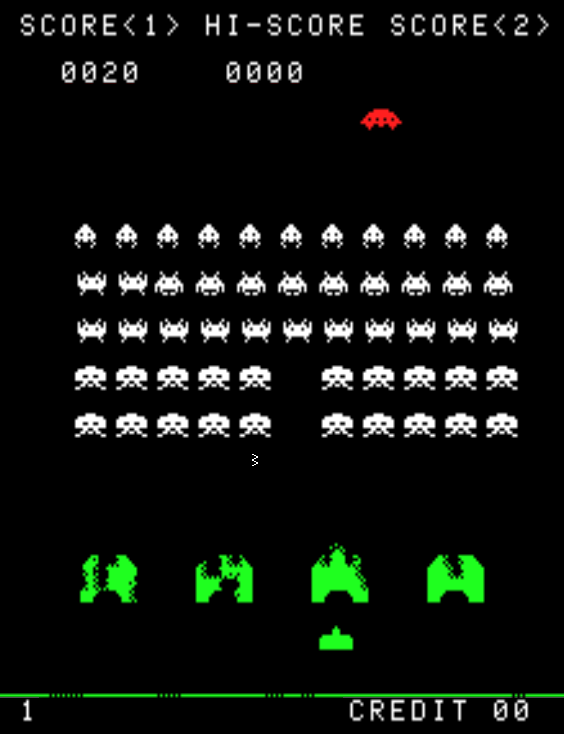
\includegraphics[scale=0.462]{images/space_game1.png}
  \end{center}
\end{figure}

Voilà ce que vous devriez trouver~:

\begin{figure}[!h]
  \begin{center}
    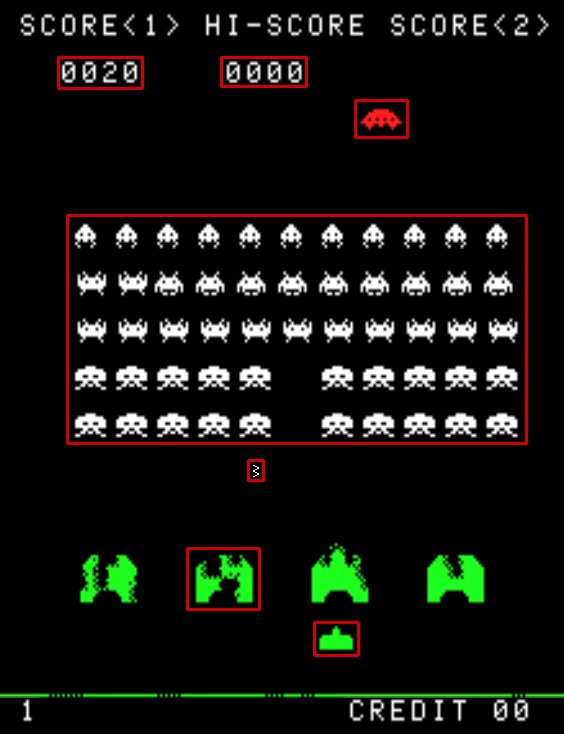
\includegraphics[scale=0.462]{images/space_game12.png}
  \end{center}
\end{figure}

Nous pouvons déjà regrouper certains objets~: les monstres et les soucoupes ont les mêmes caractéristiques. Les projectiles ascendant ou descendant sont aussi à regrouper.\\

Nous nous retrouvons donc avec les classes suivantes~:
\begin{itemize}
   \item \textbf{Monstre~:} représentant les poulpes, les crabes, les séches et les soucoupes.
   \item \textbf{Bouclier~:} empêche les projectiles de passer.
   \item \textbf{Projectile~:} ascendant ou descendant.
   \item \textbf{Joueur~:} vaisseau du joueur, \ldots
\end{itemize}

La classe \texttt{General} fait office de \emph{core engine}, elle servira à stocker les différentes instances des classes ainsi que tout ce qui ne fait parti d'aucune classe~: les scores, \ldots


\section{Quid du moteur graphique~?}

Vous avez un membre du groupe qui ne fait rien sous prétexte que la surcouche implante déjà le moteur graphique du jeu~? C'est pas aussi simple que cela.

Profitez de la boucle d'affichage \texttt{Draw} pour voir comment vous pourriez afficher un monstre, puis deux, etc.

Une fois ceci fait, n'oubliez pas que les sprites des monstres changent de manière régulière~!


\section{Que mettre dans les classes~?}

Replongez-vous une nouvelle fois dans le jeu et prennez chaque classe une par une.\\

Posez-vous les bonnes questions~: d'où vient le courant, par où passe-t-il, qu'est-ce que je cherche~?\footnote{Petite dédicace à notre cher professeur d'électronique, M. {\textsc Gabon}, pour ses questions pertinentes qui changent la vie.} En l'occurence, il n'y a pas de courant (qui a dit qu'il fallait l'imaginer \ldots?), mais que cherchez-vous concrètement~?

\subsection{La classe des monstres}

Très bien, alors que peuvent faire les monstres~?

\begin{itemize}
  \item \textbf{Ils sont distincts~:} chaque monstre a un type propre (un sprite différent entre les poulpes, les crabes et les seiches~; la soucoupe a en plus un déplacement particulier).
  \item \textbf{Ils bougent~:} il faut prévoir quelque chose pour qu'ils se déplacent, savoir où ils sont dans l'espace, vers où ils se déplacent.
  \item \textbf{Ils font gagner des points~:} c'est d'ailleurs étroitement lié à leur type\ldots
  \item \textbf{Ils peuvent être mort~:} si l'on veut afficher l'image d'explosion par exemple. Un petit quelque chose pour savoir s'il est touché peut être pratique.
  \item \textbf{Ils peuvent attaquer~:} envoyer des projectiles. Peut-être que cela serait plus adapté de faire cela dans la classe générale.
\end{itemize}

\subsection{La classe des boucliers}

En régigeant ce \tp, nous n'avons pas trouvé de manière simple de gérer les boucliers~; dans un premier temps, allez au plus simple en arrêtant tous les projectiles qui les touchent.

À partir de là, leur seul point intéressant est leur position.

\subsection{La classe des projectiles}

Que font les projectiles~?

Tout comme les monstres, ils sont \textbf{distincts} (ascendant ou descendant et des sprites différents), ont une position sur l'écran et se déplacent.

\subsection{La classe du joueur}

Le joueur représente le vaisseau en bas de l'écran. Il faut donc savoir où il se trouve, savoir le nombre de vies qu'il lui reste. Il peut également se faire toucher par des projectiles.

\subsection{La classe principale}

Elle doit stocker les données du jeu en cours. Si l'on regarde l'écran de jeu, on peut facilement faire une petite liste.\\

Que diriez-vous d'une petite liste de monstres~? Un joueur (1 dans un premier temps, puis deux~!), sans oublier cette liste de projectiles. Et pour finir un tableau de boucliers. En bonus, pourquoi pas ajouter quelques variables comme un état de pause, de menu, le nombre de pièces insérées, \ldots

Une méthode pour générer le jeu vous permettra de recommencer la partie si le joueur tue tous les monstres. N'oubliez pas d'initialiser ailleurs les autres variables~!

\helpbox{Note}{une liste est différente d'un tableau~! Une liste est dynamique alors qu'un tableau a une taille statique. Suivant votre implantation des monstres, une liste peut être plus adaptée. Elle est cependant nécessaire pour les projectiles.}

Il ne faut pas oublier d'envoyer des soucoupes de temps en temps~!


\section{Mettre à jour les données et les afficher}

\subsection{Les boucles de jeu}

Vous avez à votre disposition, dans la classe principale (\texttt{General}) deux boucles de jeu~: \texttt{Update} qui s'occupe de mettre à jour l'ensemble des données (faire bouger les monstres, faire avancer les projectiles, \ldots) et \texttt{Draw} qui se charge exclusivement de lire les données pour envoyer les objets à la surcouche.\\

Si vous regardez le premier argument passé à ces deux méthodes, il s'agit d'un intervalle de temps (\texttt{TimeStamp}). Il s'agit du temps qu'il s'est écoulé depuis le dernier appel à \texttt{Update} et respectivement \texttt{Draw}

\helpbox[vert]{Information complémentaire}{les deux boucles de jeu n'ont pas forcément le même intervalle de mise à jour. La boucle de jeu \texttt{Update} tentera de s'éxécuter le plus souvent possible, tandis que la boucle d'affichage sera appelée moins souvent afin d'être sur que le jeu s'éxécute normalement malgrès un affichage plus découpé.\\\emph{Space Invaders} est un jeu tout simple, vous ne verrez donc pas la différence, cela se ressent plus lorsque le jeu est beaucoup plus complexe et que les machines sont encore moins performantes~!}

\subsection{Mise à jour des données}

Parcourez votre liste de projectiles, une méthode \texttt{move} permettrait de les déplacer en fonction du temps écoulé depuis le dernier update. Puisqu'il est dans la nature du projectile de tuer, il peut être pratique de profiter du mouvement pour tester les collisions avec les monstres et/ou le joueur. Vous pouvez faire cela dans la même méthode ou dans une méthode séparée. Vous devrez dans les deux cas passer à votre fonction la liste de monstres et de joueur(s).\\

Utilisez l'événement \texttt{OnKeyDown} pour détecter l'appuie sur une touche fléche gauche (\texttt{Left}) ou fléche droite (\texttt{Right}). Il ne sera déclenché qu'une seule fois, pensez à sauvegarder l'état de chaque touche dans une variable que vous replacerez à sa valeur initiale lorsque l'événement \texttt{OnKeyUp} correspondant à une touche que vous attendez est déclenché.

De la même manière que vous déplacez les projectiles, une méthode pourrait permettre au vaisseau du joueur de se déplacer en fonction du temps écoulé et de la direction correspondant à la touche appuyée (et que faire lorsque les deux touches sont enfoncées~?).\\

N'oubliez pas qu'il est rare de voir un joueur avoir des vies négatives~! Et que le jeu recommence (sans effacer le score) lorsqu'il n'y a plus de monstres à tuer~!

\subsection{Affichage des sprites}

Un parcours de la liste des monstres paraît indiqué.

N'oubliez pas qu'à chaque appel de la boucle d'affichage, les éléments que vous aviez envoyé à la surcouche sont effacés. À chaque appel vous devez donc renvoyer l'ensemble des textes et textures.\\

Si vous ne savez pas comment afficher une texture, consultez la liste des méthodes graphiques utiles de la section \ref{ssec:methodutiles} page \pageref{ssec:methodutiles}.\\

Une fois que vous avez les monstres affichés sur l'écran, il ne vous sera pas plus difficile d'afficher le vaisseau du joueur, les boucliers ainsi que les projectiles.

N'oubliez pas les chaînes de caractères présentes en haut de l'écran que vous afficherez sans peine grâce à la méthode \texttt{addString}.


\section{Encore plus de précisions~?}

\subsection{Que faire lorsque l'on a plus de vie~?}

Dans un premier temps, vous pouvez simplement quitter le jeu en utilisant la méthode \texttt{quit} dans l'instance \texttt{action}.

\subsection[Autres précisions]{Vous ne trouvez pas de réponse à votre question~?}

Appelez un assistant qui attend avec enthousiasme de répondre à votre question.\\

Consultez la page d'accueil de votre serveur. Si beaucoup de questions sont répétés, il est possible que ce document soit édité et qu'une mise à jour soit publiée, peut-être que vous trouverez la réponse à votre question.

\chapter{Bonus}

Vous avez déjà terminé le jeu~? Vous pouvez y jouer, vous déplacer, tuer des monstres, perdre, \ldots~?

Ce chapitre est pour vous dans ce cas.

\section{Écrans de GameOver et menu}

Le jeu est pour l'instant jouable, mais il lui manque encore un menu et un écran de \emph{game over}.\\

Ajoutez quelques variables dans la classe principale afin de savoir si le jeu est lancé. Auquel cas, l'affichage différe entre un menu dont on doit pouvoir choisir les éléments grâce aux touches du clavier et le jeu.


\section{Envoyer les scores sur le serveur}

Comparez vos performances à Space Invaders avec vos amis en envoyant, via des requêtes HTTP vos scores en fin de partie.\\

Envoyez en utilisant la méthode POST votre score sur \url{http://etud.epita.fr/~mercie_d/GConfs/scores.php}. Le nom du champ pour indiquer le score est \texttt{score}. Envoyez avec obligatoirement le champ \texttt{game} contenant le nom de votre jeu avec sa version.

Lorsque vous gérez tout cela, vous pouvez ajouter le champ \texttt{name} qui contiendra le nom de l'utilisateur que vous demanderez sur l'écran de \emph{game over}.


\section{Réaliser un programme d'installation}

De nombreux logiciels libres vous permettent de faire ce genre de choses. En utilisant \href{http://nsis.sourceforge.net/}{Nullsoft Scriptable Install System}, vous pourrez installer les dépendances de votre projet si elles ne sont pas déjà présentes~: le framework \textsc{.net} 3.5 et \textsc{xna} 3.1.


\section{Réaliser un rapport et une présentation pour la soutenance devant les assistants}

Utilisation de \LaTeX obligatoire tant pour le rapport que pour la présentation (\href{http://lmgtfy.com/?q=beamer}{Beamer}).\\

Voici un plan type pour le rapport, le déroulement de la soutenance pourra s'inspirer du même plan~:

\begin{enumerate}
  \item Introduction
  \item Présentation de l'équipe
  \item Présentation du projet
  \item Fonctionnalités
  \item Conclusion
\end{enumerate}


\section{Recoder MAME}

\textsc{mame} est un acronyme signifiant \og Multiple Arcade Machine Emulator\fg. Il s'agit, comme son nom l'indique, un émulateur de borne d'arcade. Votre jeu n'étant pas si fidèle que ça à l'original, vous ne pourrez contentez \textit{Colona} qu'en lui proposant de rejouer au jeu original tel qu'il a été développé par Nishikado.


\section{Descent}

Arrivé à ce stade, nous vous proposons de passer au second deuxième \tp. Mais au point où vous en êtes, il n'aura pas de secret pour vous. Cela vous permettra cependant de découvrir une API 3D, mais vous en saurez plus en lisant le sujet.

\chapter{Conclusion}

Eh bien voilà, ce \tp{} touche à sa fin, vous savez maintenant utiliser \svn{} pour gérer les différentes révisions de votre projet.\\

Maintenant, il ne vous reste plus qu'à choisir le projet que vous voulez réaliser le reste de la nuit, en appliquant tout ce que l'on a vu jusqu'à présent~!

N'hésitez pas à revenir consulter ce \tp{} à chaque fois que vous en ressentez le besoin, il est important que vous maîtrisiez l'utilisation des logiciels de versionnement avant de repartir chez vous~!

% *************************
% *        annexes        *
% *************************
\appendix

\include{S_A_liens}

\include{S_A_biblio}

% *************************
% *    fin du document    *
% *************************
%\listoffigures
\end{document}